%%%%%%%%%%%%%%%%%%%%%%%%%%%%%%%%%%%%%%%%%%%%%%%%%%%%%%%%%%%%%%%%%%%%%%%%%%%%%%%%%%%%%%%%%%%%%%%%%%%%%%%%%%%%%%%%%%%%%%%%
%%%%%%%%%%%%%%%%%%%%%%%%%%%%%%%%%%%%%%%%%%%%%%%%%%                %%%%%%%%%%%%%%%%%%%%%%%%%%%%%%%%%%%%%%%%%%%%%%%%%%%%%%
%%%%%%%%%%%%%%%%%%%%%%%%%%%%%%%%%%%%%%%%%%%%%%%%%%   Prealamble   %%%%%%%%%%%%%%%%%%%%%%%%%%%%%%%%%%%%%%%%%%%%%%%%%%%%%%
%%%%%%%%%%%%%%%%%%%%%%%%%%%%%%%%%%%%%%%%%%%%%%%%%%                %%%%%%%%%%%%%%%%%%%%%%%%%%%%%%%%%%%%%%%%%%%%%%%%%%%%%%
%%%%%%%%%%%%%%%%%%%%%%%%%%%%%%%%%%%%%%%%%%%%%%%%%%%%%%%%%%%%%%%%%%%%%%%%%%%%%%%%%%%%%%%%%%%%%%%%%%%%%%%%%%%%%%%%%%%%%%%%
\documentclass[]{beamer}

\usepackage[utf8]{inputenc}
\usepackage[english]{babel}
\usepackage[T1]{fontenc}
\usepackage{textcomp}%             caractères additionnels
\usepackage{amsmath}%              pour les maths
\usepackage{amsthm}%               pour les preuves
\usepackage{amssymb}%              pour les polices maths
\usepackage{amsfonts}%             pour les polices maths
\usepackage{lmodern}%              remplacer éventuellement par txfonts, fourier, etc.

\usepackage{graphicx}%             pour inclure des images
\usepackage{listings}%             pour faire des listings de code
\usepackage{xcolor}%               pour gérer les couleurs
%\usepackage{microtype}%            améliorations typographiques que du pdflatex

\usepackage{pgf}
\usepackage{tikz}%                 pour faire des dessins avec tikzpicture
\usetikzlibrary{arrows,shapes,backgrounds,fit}

%%%% Creating handouts
% \documentclass[handout]{beamer}
% \usepackage{pgfpages}
% \pgfpagesuselayout{2 on 1}[a4paper,border shrink=5mm]

\usepackage{fancybox}

%%%%%%%%%%%%%%%%%%%%%%%%%%%%%%%%%%%%%%%%%%%%%%%%%%%%%%%
%%%%%%%%%%%%%%%%%%%% lstlistings %%%%%%%%%%%%%%%%%%%%%%
%%%%%%%%%%%%%%%%%%%%%%%%%%%%%%%%%%%%%%%%%%%%%%%%%%%%%%%
\newlength{\MaxSizeOfLineNumbers}%
\settowidth{\MaxSizeOfLineNumbers}{99}% Adjust to maximum number of lines
\addtolength{\MaxSizeOfLineNumbers}{1.5ex}%

\definecolor{darkgreen}{rgb}{0.0,0.4,0.0}%
\definecolor{darkred}{rgb}{0.8,0.0,0.0}%
\definecolor{darkcyan}{RGB}{0,139,139}
\definecolor{darkmagenta}{RGB}{139,0,139}
\definecolor{orange}{RGB}{255,127,0}

\lstdefinestyle{command} {
  language=bash,%             Langage
  inputencoding=utf8,%          Encodage
  upquote=true,%              Utilise les "quotes" correctes
  frame=shadowbox,
  rulesepcolor=\color{lightgray},%
  %framesep=1.9mm,%
  %rulesep=1mm,%
  basicstyle=\ttfamily\small,%      Style des caractères
  identifierstyle=\color{black},%     Style du code
  commentstyle=\color{black}\ttfamily,% Style des commentaires
  keywordstyle=\color{black}\ttfamily,% Style des mots clés     
  stringstyle=\color{red},%       Style des chaînes de caractères
  xleftmargin=\parindent,%        Indente à gauche selon le texte
  tabsize=2,%               Largeur d'une tabulation
  breaklines=true,%           Retour à la ligne automatique si dépassement
  %numbers=left,%
  %firstnumber=1,%
  showstringspaces=false,%        Montre les espaces dans les chaînes de caractères
  xleftmargin=\MaxSizeOfLineNumbers,%   Declarer plus haut
  % xleftmargin=15pt,%            x Rigth margin (used to align line numbers with text)
}

% Environnement pour les commandes
\lstnewenvironment{command} {%
  \lstset{
    style=command,
  }
}{}

%%%%%%%%%%%%%%%%%%%%%%%%%%%%%%%%%%%%%%%%%%%%%%%%%%%%%%%
%%%%%%%%%%%%%%%%%%%%%%% caption %%%%%%%%%%%%%%%%%%%%%%%
%%%%%%%%%%%%%%%%%%%%%%%%%%%%%%%%%%%%%%%%%%%%%%%%%%%%%%%
\usepackage{caption}%           Caption bubbles
\DeclareCaptionFont{white}{\color{white}}%
\DeclareCaptionFormat{listing}{\colorbox{darkgray}{\parbox{\dimexpr\textwidth-2\fboxsep\relax}{#1 #2#3}}}%
%\DeclareCaptionLabelFormat{listing}{\colorbox{blue}{\parbox{5cm}{#1#2}}}
%\DeclareCaptionTextFormat{listing}{\colorbox{white}{\parbox{\textwidth}{#1}}}
\captionsetup[lstlisting]{format=listing,labelfont=white,textfont=white}%
\usepackage{subcaption}%             
\usepackage{wrapfig}%
\usepackage{float}%

\def\titreEntete{Introduction of Elasticsearch}%
\def\titreShort{Elasticsearch}
%\def\ueShort{GRAR}
\def\ue{Groupe de Recherche Applications Réparties - 2014}
\def\info{Master 2 - SAR}%
%\def\titreEntete{\ue{}\\\info{}}%
\def\authorVar{Romain Pignolet}%
\def\datec{\today{}}%

\title[\titreShort{}]{\titreEntete{}}%
%\subtitle[\ueShort{}]{\ue{}\\\info{}}%
\author[\authorVar{}]{\authorVar{}}
\date[\datec{}]{\datec{}}%
\institute[Linagora]{Linagora}%

\usetheme{Boadilla}
%\usecolortheme{whale}
%%%% Available Colors
% albatross
% crane
% beetle
% dove
% fly
% seagull
% wolverine
% beaver
%%% Inner Color Themes
% lily
% orchid
% rose
%%% Outter Color Themes
% whale
% seahorse
% dolphin

%\usefonttheme{serif}
%%%% Available Font Themes
% serif
% structurebold
% structureitalicserif
% structuresmallcapsserif

% \AtBeginSection[]{
%   \begin{frame}{Contents}
%   \tableofcontents[currentsection, hideothersubsections]
%   \end{frame}
% }

\AtBeginSection[]{
  \begin{frame}{Contents}
  \tableofcontents[currentsection, hideallsubsections]
  \end{frame}
}

\begin{document}

\begin{frame}
  \titlepage
\end{frame}

\begin{frame}{Contents}
  \tableofcontents[hideallsubsections]%pausesections
\end{frame}

%%%%%%%%%%%%%%%%%%%%%%%%%%%%%
%%%%%%%%%%%%%%%%%%%%%%%%%%%%%
%%%%%%%%%%%%%%%%%%%%%%%%%%%%%
%%%%%%%%%%%%%%%%%%%%%%%%%%%%%

%%%%%%%%%%%%%%%%%%%%%%%%%%%%%%%%%%%%%%%%%%%%%%%%%%%%%%%%%%%%%%%%%%%%%%%%%%%%%%%%%%%%%%%%%%%%%%%%%%%%%%%%%%%%%%%%%%%%%%%%
%%%%%%%%%%%%%%%%%%%%%%%%%%%%%%%%%%%%%%%%%%    What is Elasticsearch ?    %%%%%%%%%%%%%%%%%%%%%%%%%%%%%%%%%%%%%%%%%%%%%%%
%%%%%%%%%%%%%%%%%%%%%%%%%%%%%%%%%%%%%%%%%%%%%%%%%%%%%%%%%%%%%%%%%%%%%%%%%%%%%%%%%%%%%%%%%%%%%%%%%%%%%%%%%%%%%%%%%%%%%%%%
\section{What is Elasticsearch ?}


\begin{frame}{\secname{}}
  \begin{itemize}
    \item Elasticsearch is a real-time distributed search and analytics engine.
    \item It is used for
    \begin{itemize}
       \item full text search
       \item structured search
       \item analytics
       \item and all three in combination
     \end{itemize}
  \end{itemize}
\end{frame}

\subsection{Who use Elasticsearch ?}

\begin{frame}{\subsecname{}}
  \begin{itemize}
    \item Wikipedia
    \item The Guardian
    \item StackOverflow
    \item GitHub
    \item Goldman Sachs
  \end{itemize}
\end{frame}

\subsection{Dependency}

\begin{frame}{\subsecname{}}
  \begin{itemize}
    \item Apache Lucene™, a full-text search engine library.
    \item Java so you need the JVM.
  \end{itemize}
\end{frame}

\subsection{Features}

\begin{frame}{\subsecname{}}
  Elasticsearch is:
  \begin{itemize}
    \item a distributed real-time document store where \textbf{every field} is indexed and searchable
    \item a distributed search engine with real-time analytics
    \item capable of scaling to hundreds of servers and petabytes of structured and unstructured data.
  \end{itemize}
\end{frame}

%%%%%%%%%%%%%%%%%%%%%%%%%%%%%%%%%%%%%%%%%%%%%%%%%%%%%%%%%%%%%%%%%%%%%%%%%%%%%%%%%%%%%%%%%%%%%%%%%%%%%%%%%%%%%%%%%%%%%%%%
%%%%%%%%%%%%%%%%%%%%%%%%%%%%%%%%%%%%%%    Installation and simple example    %%%%%%%%%%%%%%%%%%%%%%%%%%%%%%%%%%%%%%%%%%%
%%%%%%%%%%%%%%%%%%%%%%%%%%%%%%%%%%%%%%%%%%%%%%%%%%%%%%%%%%%%%%%%%%%%%%%%%%%%%%%%%%%%%%%%%%%%%%%%%%%%%%%%%%%%%%%%%%%%%%%%
\section{Installation and simples examples}

\subsection{Installation}

\begin{frame}{\subsecname{}}
  Simply download the archive on the officiel website and decompress.
\end{frame}

\subsection{Elasticsearch hierarchy}

\begin{frame}{\subsecname{}}
  The Elasticsearch folder contains:

  \begin{itemize}
    \item bin : launching scripts
    \item config : configuration files
    \item data : database location
    \item lib : library dependency
    \item logs : logs location
    \item plugins : plugins location
  \end{itemize}
\end{frame}

\subsection{Launching Elasticsearch}

\begin{frame}[containsverbatim]{\subsecname{}}
  Simply run this command:
  \begin{command}
./bin/elasticsearch
  \end{command}
\end{frame}

\begin{frame}[containsverbatim]{\subsecname{}}
  Test it out by running this command:
  \begin{command}
curl 'http://localhost:9200/?pretty'
  \end{command}

  You should see a response like this:
  \begin{command}
{
  "status" : 200,
  "name" : "Brother Nature",
  "version" : {
    "number" : "1.1.0",
    "build_hash" : "2181e113dea80b4a9e31e58e9686658a2d46e363",
    "build_timestamp" : "2014-03-25T15:59:51Z",
    "build_snapshot" : false,
    "lucene_version" : "4.7"
  },
  "tagline" : "You Know, for Search"
}
  \end{command}
\end{frame}

\subsection{Communicate with Elasticsearch}

\begin{frame}{\subsecname{}}
  There are two ways to communicate with Elasticsearch:
  \begin{itemize}
    \item Java API over port 9300
    \item Restful API with JSON over port 9200
  \end{itemize}

  Hereinafter we will discuss only about the Restful API.
\end{frame}

\subsection{How documents are stored ?}

\begin{frame}{\subsecname{}}
  \begin{itemize}
    \item Document oriented
    \item Indexes the contents of each document
    \item A document belongs to a type
    \item Types live inside an index
  \end{itemize}

  Some parallels to a traditional relational database:

  \begin{tabular}{|c|c|c|c|c|}
  \hline
  \textbf{Relational DB} & Databases & Tables & Rows & Columns\\
  \hline
  \textbf{Mongo DB} & Databases & Collections & Documents & Fields\\
  \hline
  \textbf{Elasticsearch} & Indices/Indexes & Types & Documents & Fields\\
  \hline
  \end{tabular}
\end{frame}

%%%%%%%%%%%%%%%%%%%%%%%%%%%%%%%%%%%%%%%%%%%%%%%%%%%%%%%%%%%%%%%%%%%%%%%%%%%%%%%%%%%%%%%%%%%%%%%%%%%%%%%%%%%%%%%%%%%%%%%%
%%%%%%%%%%%%%%%%%%%%%%%%%%%%%%%%%%%%%%%%%%%%%%%%    Restful API    %%%%%%%%%%%%%%%%%%%%%%%%%%%%%%%%%%%%%%%%%%%%%%%%%%%%%
%%%%%%%%%%%%%%%%%%%%%%%%%%%%%%%%%%%%%%%%%%%%%%%%%%%%%%%%%%%%%%%%%%%%%%%%%%%%%%%%%%%%%%%%%%%%%%%%%%%%%%%%%%%%%%%%%%%%%%%%
\section{Restful API}

\begin{frame}{\secname{} - Query type}
  \begin{itemize}
    \item PUT : create or update a document
    \item GET : retrieve document
    \item HEAD : check if a document exists
    \item DELETE : delete a document
  \end{itemize}

  Return
  \begin{itemize}
    \item HTTP status code (200, 404, etc.)
    \item JSON encoded body (except for HEAD requests)
  \end{itemize}
\end{frame}

\subsection{PUT Request}

\begin{frame}[containsverbatim]{\subsecname{} - Syntax}
  \begin{command}
curl -XPUT 'http://<hostname>:9200/<index>/<type>/[<id>]' -d '
{
    ...
}'
  \end{command}

  \begin{itemize}
    \item hostname : the hostname where Elasticsearch is running
    \item index : the index name
    \item type : the type name
    \item id : the ID of this particular object. If omited, the ID will be generated automatically.
  \end{itemize}
\end{frame}

\begin{frame}[containsverbatim]{\subsecname{} - Success response}
  \begin{command}
{
  "_index" : <index>,
  "_type" : <type>,
  "_id" : <id>,
  "_version" : [1..9.2e+18],
  "created" : true|false
}
  \end{command}

  \begin{itemize}
    \item \_version : Starts at 1 and increments with each update, deletes included.
    \item created : true if the PUT request create a new document.
  \end{itemize}
\end{frame}

\begin{frame}{\subsecname{} - Example}
  We want to save three documents of type employee and are in the megacorp.

  \begin{itemize}
    \item Index is "megacorp"
    \item Type is "employee"
    \item Document is an instance of "employee"
  \end{itemize}
\end{frame}

\begin{frame}[containsverbatim]{\subsecname{} - Example}
  \begin{command}
curl -XPUT 'localhost:9200/megacorp/employee/1' -d '
{
  "first_name" : "John",
  "last_name"  : "Smith",
  "age"        : 25,
  "about"      : "I love to go rock climbing",
  "interests"  : [ "sports", "music" ]
}'
curl -XPUT 'localhost:9200/megacorp/employee/2' -d '
{
  "first_name" : "Douglas",
  "last_name"  : "Fir",
  "age"        : 35,
  "about"      : "I like to build cabinets",
  "interests"  : [ "forestry" ]
}'
  \end{command}
\end{frame}

\begin{frame}[containsverbatim]{\subsecname{} - Example}
  \begin{command}
curl -XPUT 'localhost:9200/megacorp/employee/3' -d '
{
  "first_name" : "Jane",
  "last_name"  : "Smith",
  "age"        : 32,
  "about"      : "I like to collect rock albums",
  "interests"  : [ "music" ]
}'
  \end{command}
\end{frame}

\subsection{GET Request}

\begin{frame}[containsverbatim]{\subsecname{} - Syntax}
  \begin{command}
curl -XGET 'http://<hostname>:9200/<index>/<type>/<id>[/_<endpoint>][?<option1>=<value1>[&<optionN>=<valueN>...]]'
  \end{command}

  \begin{itemize}
    \item hostname : the hostname where Elasticsearch is running
    \item index : the index name
    \item type : the type name. \texttt{\_all} is a joker.
    \item id : the ID of this particular object.
  \end{itemize}
\end{frame}

\begin{frame}[containsverbatim]{\subsecname{} - Success response}
  \begin{command}
{
  "_index" : <index>,
  "_type" : <type>,
  "_id" : <id>,
  "_version" : [1..9.2e+18],
  "found": true|false,
  "_source" : {
    ...
  }
}
  \end{command}

  \begin{itemize}
    \item found : if the GET request found at least one match then \texttt{found} is true
    \item \_source : the document content only if \texttt{found} is true
  \end{itemize}
\end{frame}

\begin{frame}[containsverbatim]{\subsecname{} - Example}
  \begin{command}
curl -XGET 'localhost:9200/megacorp/employee/2?pretty'
  \end{command}

  \begin{command}
{
  "_index" : "megacorp",
  "_type" : "employee",
  "_id" : "2",
  "_version" : 1,
  "found": true,
  "_source" : {
    "first_name" : "Douglas",
    "last_name"  : "Fir",
    "age"        : 35,
    "about"      : "I like to build cabinets",
    "interests"  : [ "forestry" ]
  }
}
  \end{command}
\end{frame}

\subsubsection{Endpoint \_source}

\begin{frame}[containsverbatim]{\subsecname{} - \subsubsecname{}}
  To get just the \texttt{\_source} field of the document, without any additional content around it.

  \begin{command}
curl -XGET 'http://localhost:9200/megacorp/employee/1/_source?pretty'
  \end{command}

  \begin{command}
{
  "first_name" : "John",
  "last_name"  : "Smith",
  "age"        : 25,
  "about"      : "I love to go rock climbing",
  "interests"  : [ "sports", "music" ]
}
  \end{command}
\end{frame}

\subsubsection{Endpoint \_search}

\begin{frame}[containsverbatim]{\subsecname{} - \subsubsecname{}}
  We will search for all employees, with this request:
  \begin{command}
curl -XGET 'localhost:9200/megacorp/employee/_search?pretty'
  \end{command}

  By default, a search will return the top 10 results in the \texttt{hits} array.
\end{frame}

\begin{frame}[containsverbatim]{\subsecname{} - \subsubsecname{}}
  \begin{command}
{
  "took" : 3,
  "timed_out" : false,
  "_shards" : { ... },
  "hits" : {
    "total" : 3,
    "max_score" : 1.0,
    "hits" : [ { ... }, { ... }, { ... } ]
  }
}
  \end{command}

  Note : search includes the whole document itself in the \texttt{\_source} field.
\end{frame}

\subsubsection{Endpoint \_search with query option}

\begin{frame}[containsverbatim]{\subsecname{} - \subsubsecname{}}
  You can use the query option (\texttt{q}) to specify a simple query like:

  \begin{command}
curl -XGET 'localhost:9200/megacorp/employee/_search?q=last_name:Smith&pretty'
  \end{command}

  This query will get all employee where \texttt{last\_name} field is equal to "Smith".
\end{frame}

\subsubsection{Endpoint \_search with Query DSL}

\begin{frame}[containsverbatim]{\subsecname{} - \subsubsecname{}}
  This query use \textit{Query DSL} to do the same query as before : find all employee where last name is Smith.

  \begin{command}
curl -XGET 'localhost:9200/megacorp/employee/_search?pretty' -d '
{
  "query" : {
    "match" : {
      "last_name" : "smith"
    }
  }
}'
  \end{command}
\end{frame}

\begin{frame}[containsverbatim]{\subsecname{} - \subsubsecname{}}
  Now we will use a filter to find all employee where last name is Smith and age greater than 30.

  \begin{command}
curl -XGET 'localhost:9200/megacorp/employee/_search?pretty' -d '
{
  "query" : {
    "filtered" : {
      "filter" : {
        "range" : { "age" : { "gt" : 30 } }
      },
      "query" : {
        "match" : { "last_name" : "smith" }
      }
    }
  }
}'
  \end{command}
\end{frame}

\begin{frame}[containsverbatim]{\subsecname{} - \subsubsecname{} - Highlight search}
  Now we want to see : "Why the document matched the query ?" so we use the \texttt{highlight} parameter.

  \begin{command}
curl -XGET 'localhost:9200/megacorp/employee/_search?pretty' -d '
{
  "query" : {
    "match_phrase" : {
      "about" : "rock climbing"
    }
  },
  "highlight": {
    "fields" : {
      "about" : {}
    }
  }
}'
  \end{command}
\end{frame}

\begin{frame}[containsverbatim]{\subsecname{} - \subsubsecname{} - Highlight search}
  \begin{command}
{
  "took" : 64,
  "timed_out" : false,
  "_shards" : { ... },
  "hits" : {
    "total" : 1,
    "max_score" : 0.23013961,
    "hits" : [ { ... },
      "highlight" : {
        "about" : [ "I love to go <em>rock</em> <em>climbing</em>" ] }
    } ]
  }
}
  \end{command}

  The matched words are between \texttt{<em>} HTML tags.
\end{frame}

\subsubsection{Option \_source}

\begin{frame}[containsverbatim]{\subsecname{} - \subsubsecname{}}
  You can turn off \texttt{\_source} retrieval by using the \texttt{\_source} parameter:

  \begin{command}
curl -XGET 'http://localhost:9200/megacorp/employee/1?_source=false&pretty'
  \end{command}
\end{frame}

\begin{frame}[containsverbatim]{\subsecname{} - \subsubsecname{}}
  If you want specific fields, you can list it with \texttt{\_source} option like:

  \begin{command}
curl -XGET 'http://localhost:9200/megacorp/employee/1?_source=last_name,about&pretty'
  \end{command}

  \begin{command}
{
  "_index" : "megacorp",
  "_type" : "employee",
  "_id" : "1",
  "_version" : 1,
  "found" : true,
  "_source" : {
    "about" : "I love to go rock climbing",
    "last_name" : "Smith"
  }
}
  \end{command}
\end{frame}

\subsubsection{Endpoint \_mget}

\begin{frame}{\subsecname{} - \subsubsecname{}}
  \begin{itemize}
    \item Retrieve multiple documents with one request
    \item Reduce network overhead
    \item Faster than multiples requests
  \end{itemize}
\end{frame}

\begin{frame}[containsverbatim]{\subsecname{} - \subsubsecname{}}
  \begin{command}
curl -XGET 'http://localhost:9200/_mget?pretty' -d '
{
  "docs" : [
    { "_index" : "megacorp", "_type" :  "employee",
      "_id" : 1
    },
    { "_index" : "megacorp", "_type" :  "employee",
      "_id" : 2,
      "_source": [ "about" , "last_name" ]
    },
    { "_index" : "megacorp", "_type" :  "employee",
      "_id" : 3,
      "_source": "first_name"
    }
  ]
}'
  \end{command}
\end{frame}

\begin{frame}[containsverbatim]{\subsecname{} - \subsubsecname{} - Result}
  \begin{command}
{
  "docs" : [ {
    "_index" : "megacorp",
    "_type" : "employee",
    "_id" : "1",
    "_version" : 1,
    "found" : true,
    "_source" : {
      "first_name" : "John",
      "last_name"  : "Smith",
      "age"        : 25,
      "about"      : "I love to go rock climbing",
      "interests"  : [ "sports", "music" ]
    }
  }, { ... }, { ... } ]
}
  \end{command}
\end{frame}

\begin{frame}[containsverbatim]{\subsecname{} - \subsubsecname{} - Other syntax}
  \begin{command}
curl -XGET 'http://localhost:9200/megacorp/employee/_mget?pretty' -d '
{
  "docs" : [
    {
      "_id" : 1
    },
    {
      "_id" : 2,
      "_source": [ "about" , "last_name" ]
    },
    {
      "_id" : 3,
      "_source": "first_name"
    }
  ]
}'
  \end{command}
\end{frame}

\begin{frame}[containsverbatim]{\subsecname{} - \subsubsecname{} - Other syntax}
  \begin{command}
curl -XGET 'http://localhost:9200/megacorp/employee/_mget?pretty' -d '
{
  "ids" : [ "2", "1" ]
}'
  \end{command}
\end{frame}

\subsubsection{Endpoint \_explain}

\begin{frame}[containsverbatim]{\subsecname{} - \subsubsecname{}}
  Use to understand why one particular document matched or, more importantly, why it \textbf{didn’t match}.

  The path for the request is \texttt{/<index>/<type>/<id>/\_explain}, as in:

  \begin{command}
curl -XGET 'localhost:9200/megacorp/employee/1/_explain?pretty' -d '
{
  "query" : {
    "match" : {
      "last_name" : "smit" 
    }
  }
}'
  \end{command}
  \begin{command}
curl -XGET 'localhost:9200/megacorp/employee/1/_explain?q=last_name:smit&pretty'
  \end{command}
\end{frame}

\begin{frame}[containsverbatim]{\subsecname{} - \subsubsecname{} - Result}
  \begin{command}
{
  "_index" : "megacorp",
  "_type" : "employee",
  "_id" : "1",
  "matched" : false,
  "explanation" : {
    "value" : 0.0,
    "description" : "no matching term"
  }
}
  \end{command}
\end{frame}

\subsection{HEAD Request}

\begin{frame}{\subsecname{}}
  \begin{itemize}
    \item Return only HTTP header
    \item Document exists $\Rightarrow$ 200 OK
    \item Document not exists $\Rightarrow$ 404 Not Found
  \end{itemize}
\end{frame}

\subsection{DELETE Request}

\begin{frame}[containsverbatim]{\subsecname{}}
  If you want to remove the \texttt{megacorp} index.

  \begin{command}
curl -XDELETE 'http://localhost:9200/megacorp'
  \end{command}
\end{frame}

%%%%%%%%%%%%%%%%%%%%%%%%%%%%%%%%%%%%%%%%%%%%%%%%%%%%%%%%%%%%%%%%%%%%%%%%%%%%%%%%%%%%%%%%%%%%%%%%%%%%%%%%%%%%%%%%%%%%%%%%
%%%%%%%%%%%%%%%%%%%%%%%%%%%%%%%%%%%%%%%%%%%%%%    How it works ?    %%%%%%%%%%%%%%%%%%%%%%%%%%%%%%%%%%%%%%%%%%%%%%%%%%%%
%%%%%%%%%%%%%%%%%%%%%%%%%%%%%%%%%%%%%%%%%%%%%%%%%%%%%%%%%%%%%%%%%%%%%%%%%%%%%%%%%%%%%%%%%%%%%%%%%%%%%%%%%%%%%%%%%%%%%%%%
\section{How it works ?}

\subsection{Indexing (\_all field)}

\begin{frame}[containsverbatim]{\subsecname{}}
  \begin{itemize}
    \item All data in every field is indexed
    \item When index a document:
    \begin{enumerate}
      \item Takes all fields
      \item Concatenates them into one big string
      \item Put it in special \texttt{\_all} field
    \end{enumerate}
  \end{itemize}

  You can disable it with this mapping:

  \begin{command}
curl -XPUT 'localhost:9200/<index>/_mapping/<type>/' -d '
{
    <type>: {
        "_all": { "enabled": false }
    }
}'
  \end{command}
\end{frame}

\begin{frame}[containsverbatim]{\subsecname{} - include\_in\_all}
  Inclusion in the \texttt{\_all} field can be controlled:

  \begin{command}
curl -XPUT 'localhost:9200/<index>/<type>/_mapping/' -d '
{
    <type>: {
        "include_in_all": false,
        "properties": {
            "about": {
                "type": "string",
                "include_in_all": true
            },
            ...
        }
    }
}'
  \end{command}
\end{frame}

\subsection{Document metadata}

\begin{frame}{\subsecname{}}
  \begin{itemize}
    \item \_index : Where the document lives. (Like a Database in Relational DB)
    \item \_type : The class of object that the document represents. (Like a Table in Relational DB)
    \item \_id : The unique identifier for the document.
  \end{itemize}
\end{frame}

% \subsection{Fields}

% \begin{frame}{\subsecname{}}
  
% \end{frame}

\subsection{Types and Mappings}

\begin{frame}[containsverbatim]{\subsecname{}}
  To know the mapping for a type you can do a GET request with path: \texttt{/<index>/\_mapping/<type>}:

  \begin{command}
curl -XGET 'localhost:9200/megacorp/_mapping/employee?pretty'
  \end{command}
\end{frame}

\begin{frame}[containsverbatim]{\subsecname{}}
  \begin{command}
{
  "megacorp" : {
    "mappings" : {
      "employee" : {
        "properties" : {
          "about"      : { "type" : "string" },
          "age"        : { "type" : "long" },
          "first_name" : { "type" : "string" },
          "interests"  : { "type" : "string" },
          "last_name"  : { "type" : "string" }
        }
      }
    }
  }
}
  \end{command}
\end{frame}

\subsection{Relevance (scoring)}

\begin{frame}{\subsecname{}}
  \begin{itemize}
    \item Represented by a positive floating point number called the \texttt{\_score}
    \item The higher the \texttt{\_score}, the more relevant the document
    \item The shorter the field, the more important
    \item This distinction between field lengths disappears in the \texttt{\_all} field
  \end{itemize}
\end{frame}

%%%%%%%%%%%%%%%%%%%%%%%%%%%%%%%%%%%%%%%%%%%%%%%%%%%%%%%%%%%%%%%%%%%%%%%%%%%%%%%%%%%%%%%%%%%%%%%%%%%%%%%%%%%%%%%%%%%%%%%%
%%%%%%%%%%%%%%%%%%%%%%%%%%%%%%%%%%%%%%%%%%%%%%%%%%    Cluster    %%%%%%%%%%%%%%%%%%%%%%%%%%%%%%%%%%%%%%%%%%%%%%%%%%%%%%%
%%%%%%%%%%%%%%%%%%%%%%%%%%%%%%%%%%%%%%%%%%%%%%%%%%%%%%%%%%%%%%%%%%%%%%%%%%%%%%%%%%%%%%%%%%%%%%%%%%%%%%%%%%%%%%%%%%%%%%%%
\section{Cluster}

\subsection{Definitions}

\begin{frame}{\subsecname{}}
  \begin{definition}
    A Node:
    \begin{itemize}
      \item Is a running instance of Elasticsearch
      \item Is in a cluster
      \item Communicate with other node in the same cluster
    \end{itemize}
  \end{definition}

  \begin{figure}[h!]
    \centering
    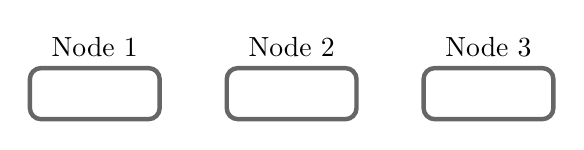
\begin{tikzpicture}
      \tikzstyle{shard}=[thick,draw=blue!75,fill=blue!20,minimum size=6mm, rounded corners]
      \tikzstyle{replica}=[thick,draw=black!75,fill=black!20,minimum size=6mm, rounded corners]
      \tikzstyle{node_master}=[draw=blue, ultra thick, inner sep=2mm, rounded corners]
      \tikzstyle{node}=[node_master, draw=black!60]
      \tikzstyle{node_text}=[draw=none, fill=none, above]

      \begin{scope}
        \node (shard1) {};
        \node (shard2) [right of=shard1] {};

        \node (node1) [node,fit=(shard1) (shard2)] {};
        \node at (node1.north) [node_text] {Node 1};
      \end{scope}

      \begin{scope}[xshift=25mm]
        \node (shard1) {};
        \node (shard2) [right of=shard1] {};

        \node (node1) [node,fit=(shard1) (shard2)] {};
        \node at (node1.north) [node_text] {Node 2};
      \end{scope}

      \begin{scope}[xshift=50mm]
        \node (shard1) {};
        \node (shard2) [right of=shard1] {};

        \node (node1) [node,fit=(shard1) (shard2)] {};
        \node at (node1.north) [node_text] {Node 3};
      \end{scope}
    \end{tikzpicture}
    \caption{Simple cluster with 3 empty nodes}
  \end{figure}
\end{frame}

\begin{frame}{\subsecname{}}
  \begin{definition}
    A Master Node:
    \begin{itemize}
      \item Is a node elected
      \item Manage cluster-wide changes like
      \begin{itemize}
        \item creating or deleting an index
        \item adding or removing a node from the cluster
      \end{itemize}
    \end{itemize}
  \end{definition}

  \begin{figure}[h!]
    \centering
    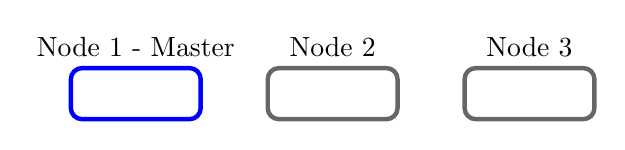
\begin{tikzpicture}
      \tikzstyle{shard}=[thick,draw=blue!75,fill=blue!20,minimum size=6mm, rounded corners]
      \tikzstyle{replica}=[thick,draw=black!75,fill=black!20,minimum size=6mm, rounded corners]
      \tikzstyle{node_master}=[draw=blue, ultra thick, inner sep=2mm, rounded corners]
      \tikzstyle{node}=[node_master, draw=black!60]
      \tikzstyle{node_text}=[draw=none, fill=none, above]

      \begin{scope}
        \node (shard1) {};
        \node (shard2) [right of=shard1] {};

        \node (node1) [node_master,fit=(shard1) (shard2)] {};
        \node at (node1.north) [node_text] {Node 1 - Master};
      \end{scope}

      \begin{scope}[xshift=25mm]
        \node (shard1) {};
        \node (shard2) [right of=shard1] {};

        \node (node1) [node,fit=(shard1) (shard2)] {};
        \node at (node1.north) [node_text] {Node 2};
      \end{scope}

      \begin{scope}[xshift=50mm]
        \node (shard1) {};
        \node (shard2) [right of=shard1] {};

        \node (node1) [node,fit=(shard1) (shard2)] {};
        \node at (node1.north) [node_text] {Node 3};
      \end{scope}
    \end{tikzpicture}
    \caption{Simple cluster with 3 empty nodes and 1 master}
  \end{figure}
\end{frame}

\begin{frame}{\subsecname{}}
  \begin{definition}
    A Shard:
    \begin{itemize}
      \item Is a low-level "worker unit"
      \item Is a single instance of Lucene
      \item Is a complete search engine
    \end{itemize}
    Our documents are stored and indexed in shards, but we don’t talk to them directly. Instead, our applications talk to an index.
  \end{definition}

  \begin{figure}[h!]
    \centering
    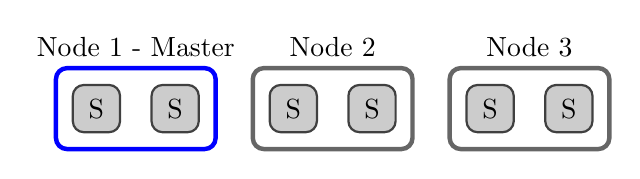
\begin{tikzpicture}
      \tikzstyle{shard}=[thick,draw=blue!75,fill=blue!20,minimum size=6mm, rounded corners]
      \tikzstyle{replica}=[thick,draw=black!75,fill=black!20,minimum size=6mm, rounded corners]
      \tikzstyle{node_master}=[draw=blue, ultra thick, inner sep=2mm, rounded corners]
      \tikzstyle{node}=[node_master, draw=black!60]
      \tikzstyle{node_text}=[draw=none, fill=none, above]

      \begin{scope}
        \node [replica] (shard1) {S};
        \node [replica] (shard2) [right of=shard1] {S};

        \node (node1) [node_master,fit=(shard1) (shard2)] {};
        \node at (node1.north) [node_text] {Node 1 - Master};
      \end{scope}

      \begin{scope}[xshift=25mm]
        \node [replica] (shard1) {S};
        \node [replica] (shard2) [right of=shard1] {S};

        \node (node1) [node,fit=(shard1) (shard2)] {};
        \node at (node1.north) [node_text] {Node 2};
      \end{scope}

      \begin{scope}[xshift=50mm]
        \node [replica] (shard1) {S};
        \node [replica] (shard2) [right of=shard1] {S};

        \node (node1) [node,fit=(shard1) (shard2)] {};
        \node at (node1.north) [node_text] {Node 3};
      \end{scope}
    \end{tikzpicture}
    \caption{Simple cluster with 3 empty nodes, 1 master and 6 shards}
  \end{figure}
\end{frame}

\begin{frame}{\subsecname{}}
  \begin{definition}
    A Primary Shard:
    \begin{itemize}
      \item Contains all documents in one index
      \item Can have other Primary Shard to spread the data (like \texttt{RAID 0})
    \end{itemize}
    The number of primary shards in an index is fixed at the time that an index is created.
  \end{definition}

  \begin{definition}
    A Replica Shard:
    \begin{itemize}
      \item Is a copy of a primary shard (like \texttt{RAID 1})
      \item Is used to provide redundant copies of your data
      \item Is used to serve read requests like searching or retrieving a document
    \end{itemize}
    The number of replica shards can be changed at any time.
  \end{definition}
\end{frame}

\begin{frame}{\subsecname{}}
  \begin{itemize}
    \item P0 : Primary Shard 0
    \item P1 : Primary Shard 1
    \item R0 : Replica Shard 0 (Copy of P0)
    \item R1 : Replica Shard 1 (Copy of P1)
  \end{itemize}

  \begin{figure}[h!]
    \centering
    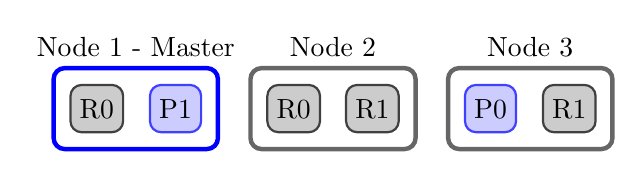
\begin{tikzpicture}
      \tikzstyle{shard}=[thick,draw=blue!75,fill=blue!20,minimum size=6mm, rounded corners]
      \tikzstyle{replica}=[thick,draw=black!75,fill=black!20,minimum size=6mm, rounded corners]
      \tikzstyle{node_master}=[draw=blue, ultra thick, inner sep=2mm, rounded corners]
      \tikzstyle{node}=[node_master, draw=black!60]
      \tikzstyle{node_text}=[draw=none, fill=none, above]

      \begin{scope}
        \node [replica] (R0-1) {R0};
        \node [shard] (P1) [right of=R0-1] {P1};

        \node (node1) [node_master,fit=(R0-1) (P1)] {};
        \node at (node1.north) [node_text] {Node 1 - Master};
      \end{scope}

      \begin{scope}[xshift=25mm]
        \node [replica] (R0-2) {R0};
        \node [replica] (R1-1) [right of=R0-2] {R1};

        \node (node2) [node, fit=(R0-2) (R1-1)] {};
        \node at (node2.north) [node_text] {Node 2};
      \end{scope}

      \begin{scope}[xshift=50mm]
        \node [shard] (P0) {P0};
        \node [replica] (R1-2) [right of=P0] {R1};

        \node (node3) [node, fit=(P0) (R1-2)] {};
        \node at (node3.north) [node_text] {Node 3};
      \end{scope}
    \end{tikzpicture}
    \caption{Simple cluster}
  \end{figure}
\end{frame}

\subsection{Node type}

\begin{frame}{\subsecname{}}
  The node can work with two parameters:
  \begin{itemize}
    \item \texttt{node.master} : if set to true, allow this node to be eligible as a master node (enabled by default)
    \item \texttt{node.data} : if set to true, allow this node to store data (enabled by default)
  \end{itemize}
\end{frame}

\begin{frame}{\subsecname{}}
  \begin{itemize}
    \item Master and Data - With default parameters, all node can be the master node and all node store data.
    \item No Master and Data (Workhorse) - This node can't become a master so it can't create index.
    \item Master and No Data (Coordinator) - This node don't store data and have free resources.
    \item No Master and No Data (Search load balancer) - This node can fetching data from nodes, aggregating results, etc.
  \end{itemize}
\end{frame}

\subsection{Cluster status}

\begin{frame}[containsverbatim]{\subsecname{}}
  \begin{command}
curl -XGET 'http://localhost:9200/_cluster/health?pretty'
  \end{command}

  \begin{command}
{
  "cluster_name":          "elasticsearch",
  "status":                "green", 
  "timed_out":             false,
  "number_of_nodes":       1,
  "number_of_data_nodes":  1,
  "active_primary_shards": 0,
  "active_shards":         0,
  "relocating_shards":     0,
  "initializing_shards":   0,
  "unassigned_shards":     0
}
  \end{command}
\end{frame}

\begin{frame}{\subsecname{}}
  The status field provides an overall indication of how the cluster is functioning:
  \begin{itemize}
    \item green: All primary and replica shards are active.
    \item yellow: All primary shards are active, but not all replica shards are active.
    \item red: Not all primary shards are active.
  \end{itemize}
\end{frame}

\subsection{Simple example}

\begin{frame}{\subsecname{}}
  \begin{itemize}
    \item Cluster with 3 Nodes
    \item One index with 2 Primary Shards
    \item Each Primary Shard has two replicas.
  \end{itemize}
  Copies of the same shard are never allocated to the same node.

  \begin{figure}[h!]
    \centering
    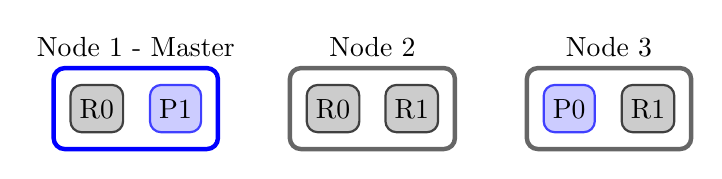
\begin{tikzpicture}
      \tikzstyle{shard}=[thick,draw=blue!75,fill=blue!20,minimum size=6mm, rounded corners]
      \tikzstyle{replica}=[thick,draw=black!75,fill=black!20,minimum size=6mm, rounded corners]
      \tikzstyle{node_master}=[draw=blue, ultra thick, inner sep=2mm, rounded corners]
      \tikzstyle{node}=[node_master, draw=black!60]
      \tikzstyle{node_text}=[draw=none, fill=none, above]

      \begin{scope}
        \node [replica] (R0-1) {R0};
        \node [shard] (P1) [right of=R0-1] {P1};

        \node (node1) [node_master,fit=(R0-1) (P1)] {};
        \node at (node1.north) [node_text] {Node 1 - Master};
      \end{scope}

      \begin{scope}[xshift=30mm]
        \node [replica] (R0-2) {R0};
        \node [replica] (R1-1) [right of=R0-2] {R1};

        \node (node2) [node, fit=(R0-2) (R1-1)] {};
        \node at (node2.north) [node_text] {Node 2};
      \end{scope}

      \begin{scope}[xshift=60mm]
        \node [shard] (P0) {P0};
        \node [replica] (R1-2) [right of=P0] {R1};

        \node (node3) [node, fit=(P0) (R1-2)] {};
        \node at (node3.north) [node_text] {Node 3};
      \end{scope}
    \end{tikzpicture}
    \caption{Simple cluster}
  \end{figure}
\end{frame}

\subsection{PUT and DELETE request (create, index and delete)}

\begin{frame}{\subsecname{}}
  \begin{figure}[h!]
    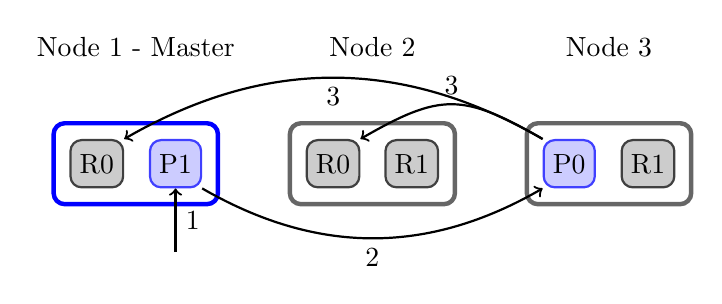
\begin{tikzpicture}
      \tikzstyle{shard}=[thick,draw=blue!75,fill=blue!20,minimum size=6mm, rounded corners]
      \tikzstyle{replica}=[thick,draw=black!75,fill=black!20,minimum size=6mm, rounded corners]
      \tikzstyle{node_master}=[draw=blue, ultra thick, inner sep=2mm, rounded corners]
      \tikzstyle{node}=[node_master, draw=black!60]
      \tikzstyle{node_text}=[draw=none, fill=none, above, yshift=7mm]
      \tikzstyle{arrow}=[thick]

      \begin{scope}
        \node [replica] (R0-1) {R0};
        \node [shard] (P1) [right of=R0-1] {P1};

        \node (node1) [node_master,fit=(R0-1) (P1)] {};
        \node at (node1.north) [node_text] {Node 1 - Master};
      \end{scope}

      \begin{scope}[xshift=30mm]
        \node [replica] (R0-2) {R0};
        \node [replica] (R1-1) [right of=R0-2] {R1};

        \node (node2) [node, fit=(R0-2) (R1-1)] {};
        \node at (node2.north) [node_text] {Node 2};
      \end{scope}

      \begin{scope}[xshift=60mm]
        \node [shard] (P0) {P0};
        \node [replica] (R1-2) [right of=P0] {R1};

        \node (node3) [node, fit=(P0) (R1-2)] {};
        \node at (node3.north) [node_text] {Node 3};
      \end{scope}

    \node (invis1) [below of=P1] {};
    \path[->] (invis1.south) edge [arrow] node [right] {1} (P1);

    \onslide<2->{\path[->] (P1.south east) edge [arrow, bend right] node [below] {2} (P0.south west);}

    \onslide<3->{\path[->] (P0.north west) edge [arrow, bend right, looseness=1.3] node [above] {3} (R0-2.north east);}
    \onslide<4->{\path[->] (P0.north west) edge [arrow, bend right] node [below] {3} (R0-1.north east);}

    \end{tikzpicture}
    \caption{PUT or DELETE request case}
  \end{figure}
\end{frame}

\subsection{GET request (retrieve)}

\begin{frame}{\subsecname{}}
  \begin{figure}[h!]
    \centering
    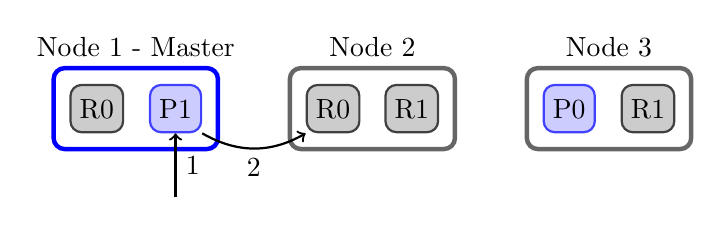
\begin{tikzpicture}
      \tikzstyle{shard}=[thick,draw=blue!75,fill=blue!20,minimum size=6mm, rounded corners]
      \tikzstyle{replica}=[thick,draw=black!75,fill=black!20,minimum size=6mm, rounded corners]
      \tikzstyle{node_master}=[draw=blue, ultra thick, inner sep=2mm, rounded corners]
      \tikzstyle{node}=[node_master, draw=black!60]
      \tikzstyle{node_text}=[draw=none, fill=none, above]
      \tikzstyle{arrow}=[thick]

      \begin{scope}
        \node [replica] (R0-1) {R0};
        \node [shard] (P1) [right of=R0-1] {P1};

        \node (node1) [node_master,fit=(R0-1) (P1)] {};
        \node at (node1.north) [node_text] {Node 1 - Master};
      \end{scope}

      \begin{scope}[xshift=30mm]
        \node [replica] (R0-2) {R0};
        \node [replica] (R1-1) [right of=R0-2] {R1};

        \node (node2) [node, fit=(R0-2) (R1-1)] {};
        \node at (node2.north) [node_text] {Node 2};
      \end{scope}

      \begin{scope}[xshift=60mm]
        \node [shard] (P0) {P0};
        \node [replica] (R1-2) [right of=P0] {R1};

        \node (node3) [node, fit=(P0) (R1-2)] {};
        \node at (node3.north) [node_text] {Node 3};
      \end{scope}

    \node (invis1) [below of=P1] {};
    \path[->] (invis1.south) edge [arrow] node [right] {1} (P1);

    \onslide<2->{\path[->] (P1.south east) edge [arrow, bend right] node [below] {2} (R0-2.south west);}

    \end{tikzpicture}
    \caption{GET request case}
  \end{figure}
\end{frame}

\subsection{Manage primary shard and replica shard}

\begin{frame}[containsverbatim]{\subsecname{}}
  Let’s create an index called \texttt{megacorp}.

  \begin{command}
curl -XPUT 'http://localhost:9200/megacorp' -d '
{
  "settings" : {
    "number_of_shards" : 3,
    "number_of_replicas" : 1
  }
}'
  \end{command}

  \begin{figure}[h!]
    \centering
    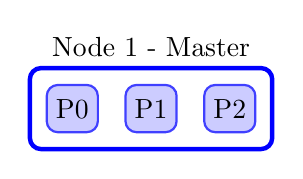
\begin{tikzpicture}
      \tikzstyle{shard}=[thick,draw=blue!75,fill=blue!20,minimum size=6mm, rounded corners]
      \tikzstyle{replica}=[thick,draw=black!75,fill=black!20,minimum size=6mm, rounded corners]
      \tikzstyle{node_master}=[draw=blue, ultra thick, inner sep=2mm, rounded corners]
      \tikzstyle{node}=[node_master, draw=black!60]
      \tikzstyle{node_text}=[draw=none, fill=none, above]

      \begin{scope}
        \node [shard] (P0) {P0};
        \node [shard] (P1) [right of=P0] {P1};
        \node [shard] (P2) [right of=P1] {P2};

        \node (node1) [node_master,fit=(P0) (P1) (P2)] {};
        \node at (node1.north) [node_text] {Node 1 - Master};
      \end{scope}

    \end{tikzpicture}
    \caption{1 node with 3 primary shards}
  \end{figure}
\end{frame}

\begin{frame}[containsverbatim]{\subsecname{}}
  Now let's check the cluster status:

  \begin{command}
curl -XGET 'http://localhost:9200/_cluster/health?pretty'
  \end{command}
  
  \begin{command}
{
  "cluster_name" : "elasticsearch",
  "status" : "yellow",
  "timed_out" : false,
  "number_of_nodes" : 1,
  "number_of_data_nodes" : 1,
  "active_primary_shards" : 3,
  "active_shards" : 3,
  "relocating_shards" : 0,
  "initializing_shards" : 0,
  "unassigned_shards" : 3
}
  \end{command}
\end{frame}

\subsection{Fault tolerance}

\begin{frame}{\subsecname{}}
  \begin{itemize}
    \item 1 Node $\Rightarrow$ Simple point of failure
    \item Solution is simple : start a new Node
    \item Node will join the cluster automatically as long as it has the same cluster name
  \end{itemize}
\end{frame}

\begin{frame}{\subsecname{}}
  \begin{figure}[h!]
    \centering
    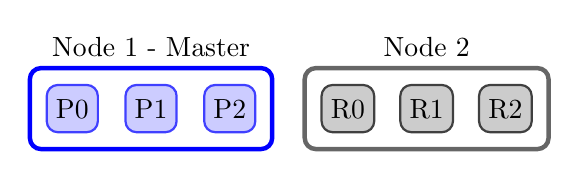
\begin{tikzpicture}
      \tikzstyle{shard}=[thick,draw=blue!75,fill=blue!20,minimum size=6mm, rounded corners]
      \tikzstyle{replica}=[thick,draw=black!75,fill=black!20,minimum size=6mm, rounded corners]
      \tikzstyle{node_master}=[draw=blue, ultra thick, inner sep=2mm, rounded corners]
      \tikzstyle{node}=[node_master, draw=black!60]
      \tikzstyle{node_text}=[draw=none, fill=none, above]

      \begin{scope}
        \node [shard] (P0) {P0};
        \node [shard] (P1) [right of=P0] {P1};
        \node [shard] (P2) [right of=P1] {P2};

        \node (node1) [node_master,fit=(P0) (P1) (P2)] {};
        \node at (node1.north) [node_text] {Node 1 - Master};
      \end{scope}

      \begin{scope}[xshift=35mm]
        \node [replica] (R0) {R0};
        \node [replica] (R1) [right of=R0] {R1};
        \node [replica] (R2) [right of=R1] {R2};

        \node (node2) [node,fit=(R0) (R1) (R2)] {};
        \node at (node2.north) [node_text] {Node 2};
      \end{scope}

    \end{tikzpicture}
    \caption{2 nodes with 3 primary shards and 1 replica shard for each primary shard}
  \end{figure}
\end{frame}

\begin{frame}[containsverbatim]{\subsecname{}}
  Wait few seconds and check the cluster status:

  \begin{command}
curl -XGET 'http://localhost:9200/_cluster/health?pretty'
  \end{command}

  \begin{command}
{
  "cluster_name" : "elasticsearch",
  "status" : "green",
  "timed_out" : false,
  "number_of_nodes" : 2,
  "number_of_data_nodes" : 2,
  "active_primary_shards" : 3,
  "active_shards" : 6,
  "relocating_shards" : 0,
  "initializing_shards" : 0,
  "unassigned_shards" : 0
}
  \end{command}
\end{frame}

\subsection{Improve performance with horizontal scaling}

\begin{frame}{\subsecname{}}
  \begin{figure}[h!]
    \centering
    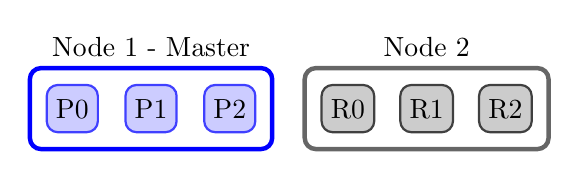
\begin{tikzpicture}
      \tikzstyle{shard}=[thick,draw=blue!75,fill=blue!20,minimum size=6mm, rounded corners]
      \tikzstyle{replica}=[thick,draw=black!75,fill=black!20,minimum size=6mm, rounded corners]
      \tikzstyle{node_master}=[draw=blue, ultra thick, inner sep=2mm, rounded corners]
      \tikzstyle{node}=[node_master, draw=black!60]
      \tikzstyle{node_text}=[draw=none, fill=none, above]

      \begin{scope}
        \node [shard] (P0) {P0};
        \node [shard] (P1) [right of=P0] {P1};
        \node [shard] (P2) [right of=P1] {P2};

        \node (node1) [node_master,fit=(P0) (P1) (P2)] {};
        \node at (node1.north) [node_text] {Node 1 - Master};
      \end{scope}

      \begin{scope}[xshift=35mm]
        \node [replica] (R0) {R0};
        \node [replica] (R1) [right of=R0] {R1};
        \node [replica] (R2) [right of=R1] {R2};

        \node (node2) [node,fit=(R0) (R1) (R2)] {};
        \node at (node2.north) [node_text] {Node 2};
      \end{scope}

    \end{tikzpicture}
    \caption{2 nodes with 3 primary shards and 1 replica shard for each primary shard}
  \end{figure}

  If we add a Node ?

  \pause

  \begin{figure}[h!]
    \centering
    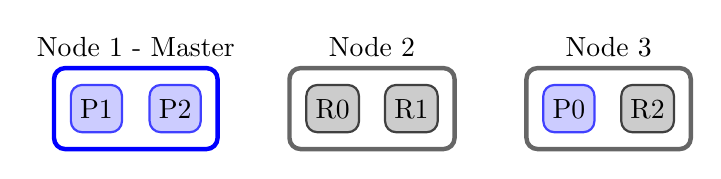
\begin{tikzpicture}
      \tikzstyle{shard}=[thick,draw=blue!75,fill=blue!20,minimum size=6mm, rounded corners]
      \tikzstyle{replica}=[thick,draw=black!75,fill=black!20,minimum size=6mm, rounded corners]
      \tikzstyle{node_master}=[draw=blue, ultra thick, inner sep=2mm, rounded corners]
      \tikzstyle{node}=[node_master, draw=black!60]
      \tikzstyle{node_text}=[draw=none, fill=none, above]

      \begin{scope}
        \node [shard] (P1) {P1};
        \node [shard] (P2) [right of=P1] {P2};

        \node (node1) [node_master,fit=(P1) (P2)] {};
        \node at (node1.north) [node_text] {Node 1 - Master};
      \end{scope}

      \begin{scope}[xshift=30mm]
        \node [replica] (R0) {R0};
        \node [replica] (R1) [right of=R0] {R1};

        \node (node2) [node,fit=(R0) (R1)] {};
        \node at (node2.north) [node_text] {Node 2};
      \end{scope}

      \begin{scope}[xshift=60mm]
        \node [shard] (P0) {P0};
        \node [replica] (R2) [right of=P0] {R2};

        \node (node3) [node,fit=(P0) (R2)] {};
        \node at (node3.north) [node_text] {Node 3};
      \end{scope}

    \end{tikzpicture}
    \caption{3 nodes with 3 primary shards and 1 replica shard for each primary shard}
  \end{figure}
\end{frame}


\begin{frame}[fragile]{\subsecname{}}
  \begin{figure}[h!]
    \centering
    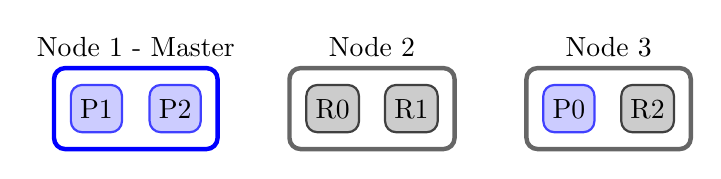
\begin{tikzpicture}
      \tikzstyle{shard}=[thick,draw=blue!75,fill=blue!20,minimum size=6mm, rounded corners]
      \tikzstyle{replica}=[thick,draw=black!75,fill=black!20,minimum size=6mm, rounded corners]
      \tikzstyle{node_master}=[draw=blue, ultra thick, inner sep=2mm, rounded corners]
      \tikzstyle{node}=[node_master, draw=black!60]
      \tikzstyle{node_text}=[draw=none, fill=none, above]

      \begin{scope}
        \node [shard] (P1) {P1};
        \node [shard] (P2) [right of=P1] {P2};

        \node (node1) [node_master,fit=(P1) (P2)] {};
        \node at (node1.north) [node_text] {Node 1 - Master};
      \end{scope}

      \begin{scope}[xshift=30mm]
        \node [replica] (R0) {R0};
        \node [replica] (R1) [right of=R0] {R1};

        \node (node2) [node,fit=(R0) (R1)] {};
        \node at (node2.north) [node_text] {Node 2};
      \end{scope}

      \begin{scope}[xshift=60mm]
        \node [shard] (P0) {P0};
        \node [replica] (R2) [right of=P0] {R2};

        \node (node3) [node,fit=(P0) (R2)] {};
        \node at (node3.north) [node_text] {Node 3};
      \end{scope}

    \end{tikzpicture}
    \caption{3 nodes with 3 primary shards and 1 replica shard for each primary shard}
  \end{figure}

  If we increase the number of replicas from 1 to 2 ?

  \pause

  \begin{command}
curl -XPUT 'http://localhost:9200/megacorp/_settings' -d ' { "number_of_replicas" : 2 }'
  \end{command}

  \begin{figure}[h!]
    \centering
    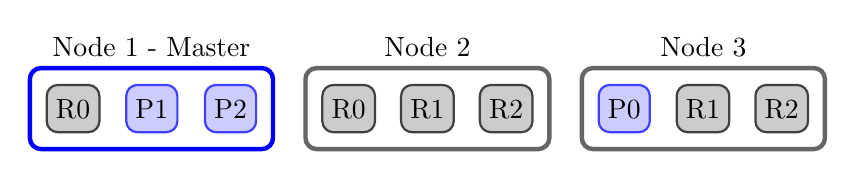
\begin{tikzpicture}
      \tikzstyle{shard}=[thick,draw=blue!75,fill=blue!20,minimum size=6mm, rounded corners]
      \tikzstyle{replica}=[thick,draw=black!75,fill=black!20,minimum size=6mm, rounded corners]
      \tikzstyle{node_master}=[draw=blue, ultra thick, inner sep=2mm, rounded corners]
      \tikzstyle{node}=[node_master, draw=black!60]
      \tikzstyle{node_text}=[draw=none, fill=none, above]

      \begin{scope}
        \node [replica] (R0) {R0};
        \node [shard] (P1) [right of=R0] {P1};
        \node [shard] (P2) [right of=P1] {P2};

        \node (node1) [node_master,fit=(R0) (P1) (P2)] {};
        \node at (node1.north) [node_text] {Node 1 - Master};
      \end{scope}

      \begin{scope}[xshift=35mm]
        \node [replica] (R0) {R0};
        \node [replica] (R1) [right of=R0] {R1};
        \node [replica] (R2) [right of=R1] {R2};

        \node (node2) [node,fit=(R0) (R1) (R2)] {};
        \node at (node2.north) [node_text] {Node 2};
      \end{scope}

      \begin{scope}[xshift=70mm]
        \node [shard] (P0) {P0};
        \node [replica] (R1) [right of=P0] {R1};
        \node [replica] (R2) [right of=R1] {R2};

        \node (node3) [node,fit=(P0) (R1) (R2)] {};
        \node at (node3.north) [node_text] {Node 3};
      \end{scope}

    \end{tikzpicture}
    \caption{3 nodes with 3 primary shards and 2 replica shards for each primary shard}
  \end{figure}
\end{frame}

\subsection{Failure case}

\subsection{Discovery}

\begin{frame}{\subsecname{}}
  \begin{itemize}
    \item Discovering nodes within a cluster
    \item Electing a master node
  \end{itemize}
\end{frame}

\subsubsection{Settings}

\begin{frame}{\subsecname{} - \subsubsecname{}}
  \begin{itemize}
    \item Use \texttt{cluster.name}.
    \item All Nodes with same \texttt{cluster.name} will be automatically in the same cluster.
  \end{itemize}
\end{frame}

\subsubsection{Discovery type}

\begin{frame}{\subsubsecname{}}
  \begin{itemize}
    \item Azure discovery
    \item EC2 discovery
    \item Google compure engine discovery
    \item Zen discovery (builtin and default)
  \end{itemize}
\end{frame}

\subsubsection{Zen discovery}

\begin{frame}{\subsubsecname{}}
  \begin{itemize}
    \item Multicast
    \item Unicast
  \end{itemize}
\end{frame}

\begin{frame}{\subsubsecname{} - Multicast}
  It provides the following settings with the \texttt{discovery.zen.ping.multicast} prefix:
  \begin{itemize}
    \item group : the group address to use. Defaults to \texttt{224.2.2.4}.
    \item port : the port to use. Defaults to \texttt{54328}.
    \item ttl (time to live) : the ttl of the multicast message. Defaults to 3.
    \item address : the address to bind to, defaults to null which means it will bind to all available network interfaces.
    \item enabled : whether multicast ping discovery is enabled. Defaults to true.
  \end{itemize}
\end{frame}

\begin{frame}{\subsubsecname{} - Unicast}
  It provides the following settings with the \texttt{discovery.zen.ping.unicast} prefix:
  \begin{itemize}
    \item hosts : Either an array setting or a comma delimited setting. Each value is either in the form of \texttt{host:port}, or in the form of \texttt{host[port1-port2]}.
  \end{itemize}
\end{frame}

%%%%%%%%%%%%%%%%%%%%%%%%%%%%%%%%%%%%%%%%%%%%%%%%%%%%%%%%%%%%%%%%%%%%%%%%%%%%%%%%%%%%%%%%%%%%%%%%%%%%%%%%%%%%%%%%%%%%%%%%
%%%%%%%%%%%%%%%%%%%%%%%%%%%%%%%%%%%%%%%%%%%    Plug it with MongoDB    %%%%%%%%%%%%%%%%%%%%%%%%%%%%%%%%%%%%%%%%%%%%%%%%%
%%%%%%%%%%%%%%%%%%%%%%%%%%%%%%%%%%%%%%%%%%%%%%%%%%%%%%%%%%%%%%%%%%%%%%%%%%%%%%%%%%%%%%%%%%%%%%%%%%%%%%%%%%%%%%%%%%%%%%%%
\section{Plug it with MongoDB}

\subsection{Prerequisites}

\begin{frame}[containsverbatim]{\subsecname{}}
  The plugin has a dependency to elasticsearch-mapper-attachment.

  \begin{command}
./bin/plugin --install elasticsearch/elasticsearch-mapper-attachments/2.0.0
  \end{command}

  Then install the river plugin:

  \begin{command}
./bin/plugin --install com.github.richardwilly98.elasticsearch/elasticsearch-river-mongodb/2.0.0
  \end{command}
\end{frame}

\subsection{Setup river plugin}

\begin{frame}[containsverbatim]{\subsecname{} - Syntax}
  \begin{command}
curl -XPUT "localhost:9200/_river/<es.river.name>/_meta" -d '
{
  "type": "mongodb",
  "mongodb": {
    "servers": [
      { "host": <mongo.instance1.host>, "port": <mongo.instance1.port> },
      { "host": <mongo.instance2.host>, "port": <mongo.instance2.port> }
    ],
    "options": { "secondary_read_preference": true },
    "db": <mongo.db.name>,
    "collection": <mongo.collection.name>
  },
  "index": {
    "name": <es.index.name>,
    "type": <es.type.name>
  }
}'
  \end{command}
\end{frame}

\begin{frame}[containsverbatim]{\subsecname{} - Example}
  \begin{command}
curl -XPUT "localhost:9200/_river/test/_meta" -d '
{
  "type": "mongodb",
  "mongodb": {
    "servers": [
      { "host": "10.75.9.193", "port": 27021 }
    ],
    "options": { "secondary_read_preference": true },
    "db": "test",
    "collection": "users"
  },
  "index": {
    "name": "usersidx",
    "type": "users"
  }
}'
  \end{command}
\end{frame}

\begin{frame}{End}
  \begin{center}
    \textcolor{red}{Thanks for your attention}
  \end{center}
\end{frame}

\end{document}